\documentclass[12pt,oneside,letterpaper]{article}
\usepackage{float}
\usepackage{graphicx}
\usepackage{varioref}
\usepackage[hidelinks]{hyperref}
\usepackage{cleveref}

% % Typeset URLs cleanly
% \usepackage{url}

% More powerful tables, incl. multi-page tables
\usepackage{longtable}
\usepackage{tabu}
% Ensure tabu tables can breathe
\global\tabulinesep=5pt


% Customization for enumerations
\usepackage{enumitem}

% Provide better unjustified text
\usepackage{ragged2e}

% Define single-spaced list
\newlist{compactenum}{enumerate}{2}
\setlist[compactenum]{label=\arabic*.,nosep}

% Define environment for single-spaced lists in tables
\newenvironment{packed_enumerate}{
  \begin{minipage}[t]{\linewidth}\begin{compactenum}[after=\strut]}
    {\end{compactenum}\end{minipage}}

% Expand the text area
\usepackage[textwidth=6.25in]{geometry}

\usepackage{titlesec}
\titleformat*{\paragraph}{\itshape}

% Set style on main pages
\pagestyle{headings}

% Set up counters for other things
\newcounter{use_case}
\crefname{use_case}{UC}{UCs}

\newenvironment{use_case}[1]{
\begin{longtabu}{|r|X|}
\hline
\refstepcounter{use_case}\label{#1}
Use Case ID & \arabic{use_case}\\
}{
\hline
\end{longtabu}
}

% Set up automatic numbering of functional requirements
\newcounter{functional_requirement}
\newcounter{tableline}
% Allow conditional statements
\usepackage{ifthen}
\newcommand{\functionalrequirementprinter}{\stepcounter{tableline}
\ifthenelse{\value{tableline}>1}{\refstepcounter{functional_requirement}
  FR-\arabic{functional_requirement}}{Requirement ID}
}
\newenvironment{func_req}{
\setcounter{tableline}{0}
\begin{longtabu}{|@{\makebox[8em][r]{\functionalrequirementprinter}}|X|}
  \hline
  Description \\
}{
\end{longtabu}
}

\title{\bfseries PolitiMap: \\
  Software Requirements Specification\\
  version 4.0}

\author {\emph{CPE 307 Group 5}\\
  \emph{California Polytechnic State University}\\
  \emph{San Luis Obispo, CA USA}}

\date{October 13, 2016}

\begin{document}
\thispagestyle{empty}\maketitle
\newpage

\tableofcontents
\newpage

\section*{Credits}
\addcontentsline{toc}{section}{Credits}
\begin{tabu}{|X[.75]|l|X|l|}
  \hline
  \textbf{Name} & \textbf{Date} & \textbf{Role} & \textbf{Version} \\
  \hline
  Alanna Buss, Andrea Savage, Kevin Pham, Frank Poole, Michael Lenz, and Dat Tran & October 5, 2015 & Authors of template document & 1.0 \\
  \hline
  Yash Mehra & October 6, 2016 & Document Owner and Author & 1.1 \\
  \hline
  Andrew Gilbert & October 6, 2016 & Author & 1.1 \\
  \hline
  Jason Yoon & October 6, 2016 & Author & 1.1 \\
  \hline
  Devon Grove & October 6, 2016 & Author & 1.1 \\
  \hline
  Matt Goodrich & October 6, 2016 & Author & 1.1 \\
  \hline
\end{tabu}

\section*{Revision History}
\addcontentsline{toc}{section}{Revision History}
\begin{tabu}{|X[L.5]|l|X|l|}
  \hline
  \textbf{Name}&\textbf{Date}&\textbf{Reason for Changes}&\textbf{Version} \\
  \hline
  Alanna Buss & October 13, 2016 & Initial format for requirements document & 1.0 \\
  \hline
  Yash Mehra & October 13, 2016 & Added introduction content and updated formatting & 2.0 \\
  \hline
  Jason Yoon & October 13, 2016 & Added Use Cases & 2.1 \\
  \hline
  Jason Yoon and Matt Goodrich & October 14, 2016 & Added Flowchart & 2.2 \\
  \hline
  Yash Mehra & October 14, 2016 & Added System Requirements & 2.3 \\
  \hline
  Yash Mehra & October 14, 2016 & Added Non-Functional Requirements and External Interface Requirements & 2.4 \\
  \hline
  Yash Mehra & October 14, 2016 & Fixed Use Cases formatting & 3.0 \\
  \hline
  Jason Yoon & October 14, 2016 & Fixed External Interface Requirements and UI Requirements& 3.1 \\
  \hline
  Andrew Gilbert & October 14, 2016 & Added my use case and tweak formatting & 3.2 \\
  \hline
  Andrew Gilbert & October 14, 2016 & Proofreading and corrections. & 3.3\\
  \hline
  Andrew Gilbert & October 15, 2016 & Spelling, grammar, and structure review. Final check for submission. & 4.0 \\
  \hline
  Devon Grove & October 15, 2016 & Customer Segment improvements and additional proofreading. & 4.1 \\
  \hline
\end{tabu}

\newpage

\section{Introduction}
\subsection{Purpose}
This Software Requirements Specification describes the functional and
nonfunctional software requirements for an application that brings
local, regional and national political information to a user's mobile
device.  This document is intended to be used by the members of the
project team who will implement and verify the correct functionality
of the system. This document will also be viewed by our professor,
Dr. Clark Turner.

\subsection{Intended Audience and Reading Suggestions}

\subsubsection{Software Development Engineers}
Developers will primarily reference the functional and nonfunctional
requirements. These requirements correspond to the features to be
implemented. For the purposes of implementation, it may also be
helpful to reference use cases.

\paragraph{Suggested Reading Sequence:}
\begin{compactenum}
\item Overall Description
\item System Features
\item Use Cases
\item External Interface Requirements
\item Other Nonfunctional Requirements
\end{compactenum}

% I don't think we have any owners or customers besides ourselves
% right now --AG
% I am including some information about our targeted customer
% archetype for now. This is supposed to be intended audience, not
% active audience. --DG
\subsubsection{Software Product Owners and Customers}
The user segment served by this project is the citizen and legislator population of
the City of San Luis Obispo, California. Within this user segment
exists two primary demographics: a user base between the ages of 35 and 50
(middle-aged), and a user base between the ages of 18 and 22 (college students
at California Polytechnic State University.
% Customers will observe and confirm that the specified features and
% requirements meet business needs and that all user needs are brought
% to attention. Additionally, they will serve as the primary product
% owner as they will prioritize features during implementation.

% \paragraph{Suggested Reading Sequence:}
% \begin{compactenum}
% \item Overall Description
% \item System Features
% \item Use Cases
% \item External Interface Requirements
% \item Other Nonfunctional Requirements
% \end{compactenum}

\subsection{Project Scope}
Initially, the application's only function will be to view current
bills in the San Luis Obispo City Council.

Following a successful initial release, following releases are
expected to add the ability to display current bills in the San Luis
Obispo County Supervisors, followed by the California State
Legislature and the US Congress. Push notifications will be added to
notify users when a new bill is introduced. Further expansion to
cover more geographical locations would be possible.

\subsection{References}
\begin{compactenum}
\item Vision and Scope\\
  \url{https://docs.google.com/document/d/1hyrRutAoTPR2VO-z9vAM3607bGrHKqxODCZUUu3c8WM/edit}
\end{compactenum}

\section{Overall Description}
\subsection{Product Perspective}
The application will provide local, regional and national political
information based on the address provided by the user. The information
will be displayed in an uncluttered, readable, and simple format.
User-preferred locations will be able to be saved, edited, and deleted.

\subsection{Product Features}
\subsection{User Classes and Characteristics}
\begin{longtabu}{|l|X|}
  \hline
  \textbf{User Class}&\textbf{Description}\\
  \hline
  Local voters & View bills that may affect them and when such bills will be up for vote. View bills at different levels of government.\\
  \hline
  Local activist groups & Make bills affecting their causes more widely known. Finding and supporting politicians who support their position.\\
  \hline
  Local government officials & Will likely receive more calls from voters if the application succeeds. Not direct users of the application, but directly affected by the popularity of the application. In later versions of the application, may be able to notify users of requests for public comment.\\
  \hline
\end{longtabu}

\subsection{Operating Environment}
This project will produce an iPhone mobile application aimed at
users across the United States. Since our initial target audience is
limited to a domestic one, the geographic distribution will not be such
that servers at multiple locations will be necessary. Instead, the
application will request relevant information using REST calls to a
backend that provides the information in JSON format.

All information will be stored in JSON files since the data is static
and read-only. Given the scope of this project, a secure database is
unnecessary and setting one up is a waste of resources.  Should the
application evolve into an interactive one, a database should not be
difficult to retrofit, as our backend will be serving JSON via HTTP GET
calls, which can be generated from a database just as easily.
% I don't like the wording of that last sentence---should I just leave
% it out, or how can it be reworded?

At this stage, we have not explored revenue streams for our business
model besides advertising. At present, allowing user access for free
reduces our obligation to users, avoiding some of the potential
consequences of a major service outage. We do not anticipate server
load to be unbearable, as we expect PolitiMap to be accessed only once
or twice a day per user.

\subsection{Design and Implementation Constraints}
\begin{enumerate}
\item The initial version of the mobile application will be ported to
the iPhone App Store only, as it will be written in Swift.
\item The initial backend data will exist as static JSON files
  served from a web server.
\end{enumerate}

\subsection{User Documentation}
TBD

\subsection{Assumptions and Dependencies}
\subsubsection{Assumptions}
\begin{enumerate}
\item Voter involvement with local politics is poor.
\item Increased involvement with local politics is beneficial.
\item Voters lack information in order to be more involved with local politics.
\item The rationale for poor voter turnout is local political ignorance.
\end{enumerate}

\subsubsection{Dependencies}
\begin{enumerate}
\item Ability to get data on bills in a machine-parsable format (even if that is initially plaintext with custom code to parse it)
\end{enumerate}

\section{Use Cases}
\subsection{User Stories}
\begin{longtabu}{|r|X|}
  \hline
  Case ID & Description \\
  \hline
  \cref{locations} & As a frequent traveler, I want to be able to save
  multiple locations within the app so I can easily access the
  information on where I travel the most. \\
  \hline
  \cref{policies} & As a Cal Poly student, I want to be able to view
  policy positions of local politicians so I can become encouraged to
  participate in local politics and make informed decisions in local
  elections. \\
  \hline
  \cref{past_bills} & As a new voter, I want to be able to view
  previously-passed bills, so I can understand how politics have evolved
  and develop context for future bills. \\
  \hline
  \cref{international} & As an international student who is not
  familiar with US politics, I want to be able to pinpoint bills that
  influence me, so I can be aware of my political position.\\
  \hline
  \cref{agendas} & As a Cal Poly student, I want to be able to
  find the agenda for the city council meeting
  tonight so I can make my voice heard. \\
  \hline
\end{longtabu}


\begin{use_case}{locations}
  Use Case Name & Save Locations\\
  Created By & Yash Mehra\\
  Last Updated By & Andrew Gilbert\\
  Date Created & 2016-10-06\\
  Date Last Updated & 2016-10-15\\
  Actors & The PolitiMap App\\
  Description & Save multiple locations on the home page of the application\\
  Preconditions &
  \begin{packed_enumerate}
  \item The location is currently supported by the app
  \item The app is open
  \item The app is on the home page
  \end{packed_enumerate} \\
  Postconditions &
  \begin{packed_enumerate}
  \item The app shows the saved location on the home page.
  \item The app should be able to access the location and show its political information when tapped
  \end{packed_enumerate} \\
  Normal Flow &
  \begin{packed_enumerate}
  \item The user opens app
  \item (Alternative flow 1)
  \item The app loads locations saved by the user
  \item The user views saved locations
  \end{packed_enumerate} \\
  Alternative Flows &
  Alternative flow 1

  \begin{packed_enumerate}
  \item The user searches a new locations
  \item The user chooses to save the location
  \end{packed_enumerate} \\
  Priority & High\\
  Special Requirements & \\
  Assumptions & All locations can be found\\
\end{use_case}

\begin{use_case}{policies}
  Use Case Name & Display Policy Positions\\
  Created By & Devon Grove\\
  Last Updated By & Andrew Gilbert\\
  Date Created & 2016-10-07\\
  Date Last Updated& 2016-10-15\\
  Actors & The PolitiMap App\\
  Description & View policy summary of given local politician on active issues\\
  Preconditions &
  \begin{packed_enumerate}
  \item The user's location is currently supported by the app
  \item The user has chosen the city council member to evaluate
  \item The user has selected ``Policy Positions'' from menu options
  \end{packed_enumerate} \\
  Postconditions &
  \begin{packed_enumerate}
  \item The app displays a summarized list of policy positions on
    active local legislation, and lists a ``position not available''
    message if position is indeterminate
  \end{packed_enumerate} \\
  Normal Flow &
  \begin{packed_enumerate}
  \item The user opens the app
  \item The user specifies their location, or a cached location is processed
  \item The user selects ``Politicians'' from the lower UI menu
  \item The user selects their chosen politician from the ``Your Representatives'' list
  \item The user navigates to ``Policy Positions'' using the UI menu
  \end{packed_enumerate} \\
  Priority & Medium\\
  Special Requirements & None\\
  Assumptions & Policy positions will be available publicly through government or council member's website\\
\end{use_case}

\begin{use_case}{past_bills}
  Use Case Name&View Federal Bills\\
  Created By&Matthew Goodrich\\
  Last Updated By&Andrew Gilbert\\
  Date Created&October 6, 2016\\
  Date Last Updated&October 15, 2016\\
  Actors&
  \begin{packed_enumerate}
  \item The Application User
  \item The PolitiMap App
  \item The Backend Server
  \end{packed_enumerate}\\
  Description&The application shall display a list of federal bills and further information about each upon selection.\\
  Preconditions&
  \begin{packed_enumerate}
  \item The device is connected to the internet.
  \item The backend is loaded with the organized data.
  \item The device has the application downloaded, updated, and open to the home screen.
  \item The backend server is running, whether it be an AWS component or EC2 instance.
  \end{packed_enumerate}\\
  Postconditions&
  \begin{packed_enumerate}
  \item A list of federal bills will be shown and likely scrolled-down, or the details of a specific bill will be showing.
  \item A request will have been made to the AWS component or EC2 instance.
  \item TBD - The federal bills may be cached in the user's device.
  \end{packed_enumerate}\\
  Normal Flow&
  \begin{packed_enumerate}
  \item The user chooses to view the list of bills relating to their local, state, and federal governments.
  \item A GET request is made to the web server while the user sees a loading animation.
  \item The user selects to filter the list of bills to show only federal bills.
  \item The user scrolls through the bills and notices an interesting one.
  \item The interesting bill is selected and the user reads related information, including a summary, associated representatives, and links to related external documentation.
  \end{packed_enumerate}\\
  Alternative Flow&
  \begin{packed_enumerate}
  \item The user selects a federal bills list instead of filtering a combined list.
  \item The bills are loaded upon opening the application and only refreshed manually.
  \item The bill information does not include associated representatives.
  \item The bill shows dynamic data, such as votes and comments.
  \end{packed_enumerate}\\
  Exceptions&
  \begin{packed_enumerate}
  \item Unable to load the bills through the lack of an internet connection.
  \end{packed_enumerate}\\
  Includes&
  \begin{packed_enumerate}
  \item An external library to make the GET request.
  \end{packed_enumerate}\\
  Priority&High - One of the core functions of the application.\\
  Frequency of Use&Depends on the number of users and other variables.\\
  Business Rules&None\\
  Special Requirements&
  \begin{packed_enumerate}
  \item The application requests the data asynchronously.
  \item The device is an iPhone 5 or newer.
  \item Specific bill information is loaded with a GET request after a bill is selected.
  \end{packed_enumerate}\\
  Assumptions&
  \begin{packed_enumerate}
  \item Viewable federal bills exist in the backend.
  \item Representatives have been linked to associated bills.
  \item Documentation links have been added to associated bills.
  \end{packed_enumerate}\\
  Notes and Issues&None\\
\end{use_case}

\begin{use_case}{international}
  Use Case Name & View bills that influence foreign students \\
  Created By & Jason Yoon \\
  Last Updated By & Andrew Gilbert \\
  Date Created & October 6, 2016 \\
  Date Last Updated & October 15, 2016 \\
  Actors &
  \begin{packed_enumerate}
  \item The Politimap App
  \item The Backend Server
  \end{packed_enumerate}\\
  Preconditions&
  \begin{packed_enumerate}
  \item The device is connected to the internet and the app is downloaded.
  \item The app is opened showing the main page.
  \end{packed_enumerate}\\
  Postconditions&
  \begin{packed_enumerate}
  \item One of the menus should direct the user to a new page.
  \item The page will contain bills that are related to foreign students.
  \end{packed_enumerate}\\
  Normal Flow &
  \begin{packed_enumerate}
  \item The user opens the app
  \item The user navigates to the menu where it says ``foreign students''
  \item The user is able to scroll through the list of bills and save them in the bookmark
  \end{packed_enumerate}\\
  Alternative Flow & None \\
  Special Requirements & None \\
  Priority & Low \\
\end{use_case}

\begin{use_case}{agendas}
  Use Case Name & Display Agenda\\
  Created By & Andrew Gilbert\\
  Last Updated By & Andrew Gilbert\\
  Date Created & 2016-10-06\\
  Date Last Updated & 2016-10-15\\
  Actors & The PolitiMap App\\
  Description & Display the agenda for the next City Council meeting\\
  Preconditions &
  \begin{packed_enumerate}
  \item The user has chosen a location which has a city council
  \item The location is currently supported by the app
  \item The app is open
  \item The user has chosen ``City Council Meeting'' from the list of events.
  \end{packed_enumerate} \\
  Postconditions &
  \begin{packed_enumerate}
  \item The app shows the agenda for the next City Council meeting for
    the selected location.
  \end{packed_enumerate} \\
  Normal Flow &
  \begin{packed_enumerate}
  \item The user opens app
  \item The app requests data from server
  \item (Alternative flow 1)
  \item The app displays a list of upcoming events
  \item The user chooses the City Council item
  \end{packed_enumerate} \\
  Alternative Flows &
  Alternative flow 1

  \begin{packed_enumerate}
  \item Read data from cache
  \end{packed_enumerate} \\
  Priority & High\\
  Special Requirements & None\\
  Assumptions & Council meeting agendas will be available for all
  supported locations\\
  Notes and Issues & None\\
\end{use_case}

\section{Flowchart}
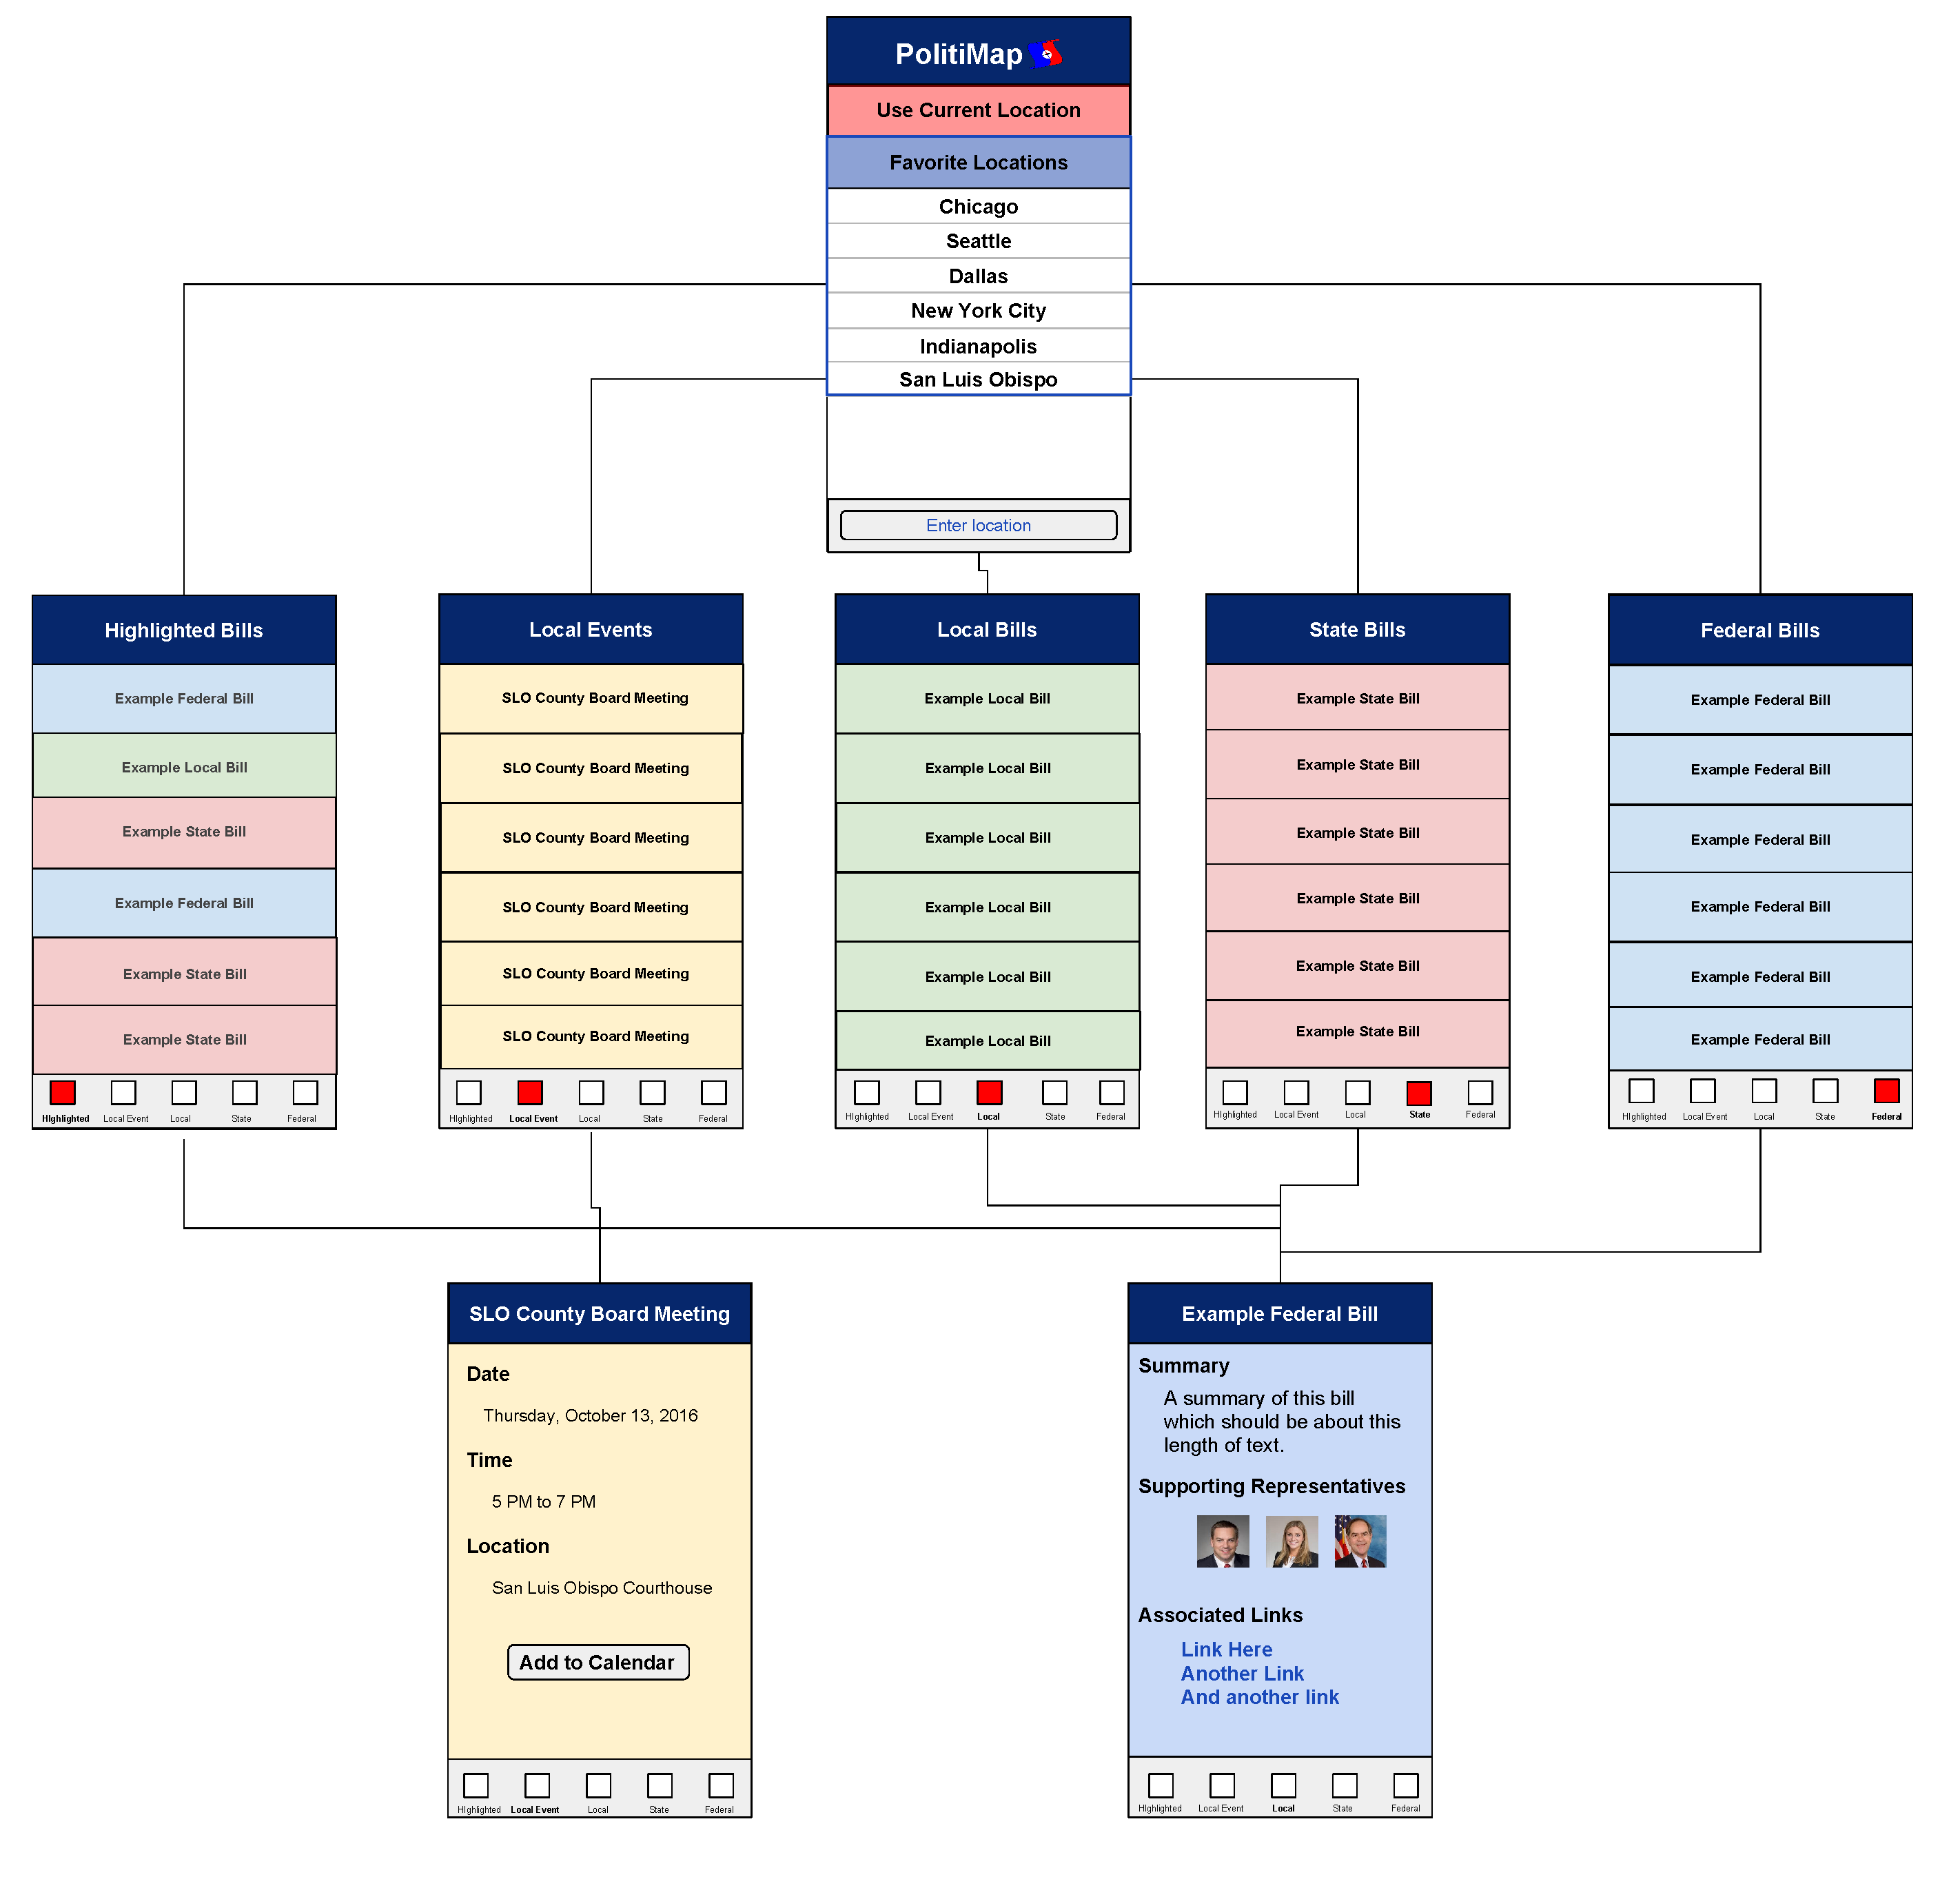
\includegraphics[width=\textwidth]{flowchart.pdf}

\section{System Features}

\subsection{Data Transmission}
\subsubsection{Description and Priority}
The data format must be standardized for each location level: local, regional,
and national. Data must be available to the system every time a call
is made.

\subsubsection{Stimulus/Response Sequences}
\begin{longtabu}{|r|X|}
  \hline
  Stimulus & Once a location has been provided and the user has accessed it, the application will make a REST API call to the back end framework.\\
  \hline
  Response & The system will provide the data in the specified JSON format as a response to the REST API call.\\
  \hline
\end{longtabu}
\subsubsection{Functional Requirements}
\begin{func_req}
  \hline
  The system shall load data in the JSON format specified in an appendix (TBD). \\
  \hline
  The system shall fetch the data using REST. \\
  \hline
  The system shall only load JSON data for the locations
  selected by the user. \\
  \hline
  The data on politicians shall be verifiable and completely accurate.\\
  \hline
\end{func_req}

\subsection{Address Setting}
\subsubsection{Description and Priority}
The system will store the saved and preferred locations on the user's
device. The address of the location and information about its
associated governmental levels will be stored. The address information
stored can be manipulated by the user.
\subsubsection{Stimulus/Response Sequences}
\begin{longtabu}{|r|X|}
  \hline
  Stimulus & The application is on the home page and the user searches for a new address. \\
  \hline
  Response & The application verifies location, queries the server for associated governmental levels, and stores the new information. \\
  \hline
\end{longtabu}
\subsubsection{Functional Requirements}
\begin{func_req}
  \hline
  The system shall have local storage mechanisms for stored user locations. \\
  \hline
  The system shall be able to read and write new data to the local storage mechanism according to the user's preference. \\
  \hline
\end{func_req}

\subsection{Address editing}
\subsubsection{Description and Priority}
The user information is under the user's full control. The user should
be able to add, edit and delete any user information. Users will not
be able to edit the requested data from saved locations, only the
addresses of saved locations.
\subsubsection{Stimulus/Response Sequences}
\begin{longtabu}{|r|X|}
  \hline
  Stimulus & User chooses to edit address. \\
  \hline
  Response & Option to change address or delete it completely from the application. \\
  \hline
\end{longtabu}
\subsubsection{Functional Requirements}
\begin{func_req}
  \hline
  The system shall store user locations only on the user's device. \\
  \hline
  The system shall not allow the users to edit the information received from the server about bills.\\
  \hline
  The system shall not allow the users to edit the information stored on the server about bills.\\
  \hline
\end{func_req}

\section{External Interface Requirements}
\subsection{User Interfaces}
For additional information about user interfaces, refer to the
flowchart above.
\begin{longtabu}{|r|X|}
  \hline
  UI Requirement & Description \\
  \hline
  UI-1 & The homepage will display a list of favorite locations and a search bar. It will also display a menu to search based on the current location. \\
  \hline
  UI-2 & The ``Highlighted Bills'' page will display a list of highlighted bills at the Local, State, and Federal levels of government. At the bottom of the page, it will display tabs that link to other pages. It will also indicate the current page. \\
  \hline
  UI-3 & The ``Local Events'' page will display a list of local events. At the bottom of the page, it will display tabs that link to other pages. It will also indicate the current page. \\
  \hline
  UI-4 & The ``Local Bills'' page will display a list of local bills. At the bottom of the page, it will display tabs that link to other pages. It will also indicate the current page.\\
  \hline
  UI-5 & The ``State Bills'' page will display a list of state bills. At the bottom of the page, it will display tabs that link to other pages. It will also indicate the current page.\\
  \hline
  UI-6 & The ``Federal Bills'' page will display a list of federal bills. At the bottom of the page, it will display tabs that link to other pages. It will also indicate the current page.\\
  \hline
  UI-7 & The ``Description'' page will display the details of the selected item. It will also display tabs that link to other pages. \\
  \hline
\end{longtabu}

\subsection{Hardware Interfaces}
The only hardware interface requirement is induced by the software interface requirements:
\begin{longtabu}{|r|X|}
  \hline
  HI Requirement & Description \\
  \hline
  HI-1 & The user device must be an iPhone 5 or newer.\\
  \hline
\end{longtabu}

\subsection{Software Interfaces}
\begin{longtabu}{|r|X|}
  \hline
  SI Requirement & Description \\
  \hline
  SI-1 & The user OS must be iOS.\\
  \hline
  SI-2 &  The user system shall have access to the Apple App Store. \\
  \hline
  SI-3 & The application shall be updated through the Apple App Store.\\
  \hline
  SI-4 & The application shall be written in Swift.\\
  \hline
\end{longtabu}

\section{Other Nonfunctional Requirements}
\subsection{Performance Requirements}
\begin{longtabu} {|r|X|}
  \hline
  PR-1 & The system shall load each page in under 2 seconds. \\
  \hline
  PR-2 & The system shall have zero memory leaks. \\
  \hline
  PR-3 & All bills will be updated within 1 day of receiving new information. \\
  \hline
\end{longtabu}

\subsection{Security Requirements}
\begin{longtabu}{|r|X|}
  \hline
  CR-1 & User location information shall be secure.\\
  \hline
\end{longtabu}

\subsection{Software Quality Attributes}
\begin{longtabu} {|r|X|}
  \hline
  SQ-1 & The system tests shall be repeatable\\
  \hline
\end{longtabu}
\end{document}
% LocalWords:  PolitiMap
